\chapter{Reinforcement Learning Algorithms and Tools}\label{chapter:reinforcement_learning}

In this chapter, we will dig deeper into Reinforcement Learning algorithms. How they algorithms are implemented, what are their strengths and weaknesses? We will present our state-of-art algorithm, SAC (Soft-Actor-Critic), and the algorithm we want to test on the robotics applications, BDQ (Branched-Dueling Q-learning). We will mention the fundamental differences between those two algorithms—for instance, their optimization objective functions, and different exploration approaches. 

After the introduction of algorithms, we are going to present RL environment frameworks and algorithm libraries. We base our custom robotics environment on Gym environment definition. In the same way, we intensively used open-source RL baseline algorithm library called Stable-Baselines. For the implementation of neural networks, we imported Tensorflow and Keras. Finally, we introduce Optuna as our hyper-parameter optimization tool. 

Overall we depend on a lot of different software libraries, which we don’t mention here; the interested audience can take a look at our Github page\footnote{\url{https://bit.ly/3k8uSga}}.

\section{Soft Actor Critic (SAC)}


SAC algorithm is described as the state-of-art algorithm as of 2020 \cite{stable-baselines}. Therefore, we chose SAC as our baselines algorithm to compare against the BDQ. SAC is an actor-critic, model-free algorithm. Actor critic refers to the optimization of both policy and value function. Model-free nature stems from the sample based update structure. The success of SAC lies in low sample complexity and robustness to different hyperparameters \cite{Haarnoja2018}. SAC achieved this success due to; actor-critic architecture, entropy maximization, and off-policy update structure.

% \todo{elaborate more on actor-critic}

Actor-critic architectures have long been used in RL literature \cite{Konda2000}. \cite{Haarnoja2018}. The actor-critic's core idea is optimizing the policy and value functions separately but combining them during the policy iteration part of the RL algorithm. The policy function is responsible for the policy evaluation, while the value function is responsible for policy improvement.


\begin{equation}
    \pi^*_{MaxEnt} = \arg\max_{\pi}\sum_t\mathop{\mathbb{E}}_{(s_t,a_t)\sim \rho_{\pi}}[r(s_t, a_t) + \alpha H(\pi(.|s_t))]
    \label{eq:maxentRL}
\end{equation}

\begin{equation}
    H(X) = \mathop{\mathbb{E}}_X [I(x)] = -\sum\limits_{x \in X} p(x)\log p(x)
\end{equation}

Off-policy, algorithms are naturally better at working in the sparse data region because they can incorporate past experiences and use state-action-rewards pairs from different policies.  Albeit the off-policy approach brings high variance into the learning process, new papers overcome this problem with Polyak-Rupper averaging or adaptively setting the step size of the stochastic gradient descent optimizer \cite{Sutton2018}.

\subsection{SAC Implementation as Baseline Algorithm}

We use the stable-baselines implementation of the SAC algorithm. This implementation uses double soft-Q functions, a soft-state value function to estimate the critic, and a policy network to estimate the actor. Stable-baselines supports automatically learning the entropy coefficient. This feature saves the user time by avoiding hand-tuning on the entropy coefficient term.

Unlike the tabular soft-policy iteration method, where policy evaluation and policy iteration steps follow each other strictly, soft-actor-critic calculates the losses of both critic and actor update the parameters by stochastic gradient descent in one iteration. Although the function approximator implementation of SAC does not directly follow the policy-iteration, it inherently follows the generalized policy iteration schema. 

The essential characteristic of SAC is the entropy maximization. The entropy bonus comes into play when calculating the bellman backup of soft-Q-function, soft-state value function, and the policy loss. That means the learned policy must maximize the rewards and entropy at the same time. 

The soft Q-function loss is represented in the equation below \ref{eq:softqfuncloss}, which is the same loss function used by Mnih et al. in 2015, updates the parameters of the Q-network in the direction of the TD target. The only difference in the Q-function update step between SAC and DQN is the inclusion of entropy variables in the state-value network \ref{eq:statevalueloss}.

\begin{equation}
    V(s_t) = \mathop{\mathbb{E}}_{a_t \sim \pi}[Q(s_t,a_t)- \alpha \log \pi(a_t|s_t)]
    \label{eq:statevalueloss} 
\end{equation} 

\begin{equation}
    \pi_{new} = \arg\min\limits_{\pi' \in \Pi} \Bigg(\pi'(.|s_t) \Bigg|\Bigg| \frac{exp(\frac{1}{\alpha} Q^{\pi_{old}}(s_t,.))}{Z^{\pi_{old}}(s_t)} \Bigg)
\end{equation}

\begin{equation}
    J_Q(\theta) = \mathop{\mathbb{E}}_{(s_t,a_t)\sim D} \Big[ \frac{1}{2}(Q_{\theta}(s_t,a_t)-(r(s_t,a_t) + \gamma \mathop{\mathbb{E}}_{(s_t,a_t)\sim p}[V_{\theta^-}(s_{t+1})]))^2 \Big]
    \label{eq:softqfuncloss}
\end{equation}

SAC and DQN diverge in the policy improvement step, where DQN updates the policy based-on epsilon-greedy approach, SAC parameterizes the policy with a neural network and updates the parameters in the direction of the minimum loss function \ref{eq:losspolicy}. Haarnoja et al. manipulate the policy definition with a reparameterization trick to allow stochastic descent on the loss function \ref{eq:reparameterization}.

\begin{equation}
    J_{\pi}(\phi) = \mathop{\mathbb{E}}_{s_t \sim D, \epsilon \sim N} \Big[\alpha \log\pi_{\phi}(f_{\phi}(\epsilon_t;s_t)|s_t) - Q_{\theta}(s_t, f_{\phi}(\epsilon_t;s_t))\Big]
    \label{eq:losspolicy}
\end{equation}

\begin{equation}
    a_t = f_{\phi}(\epsilon_t; s_t)
    \label{eq:reparameterization}
\end{equation} 

The soft Actor-Critic algorithm given in \ref{fig:sacalgo} follows the general guidelines of actor-critic type of algorithms with the introduction of entropy maximation RL into the definitions of Q and policy functions.

\begin{figure}[htbp] 
    \centering
    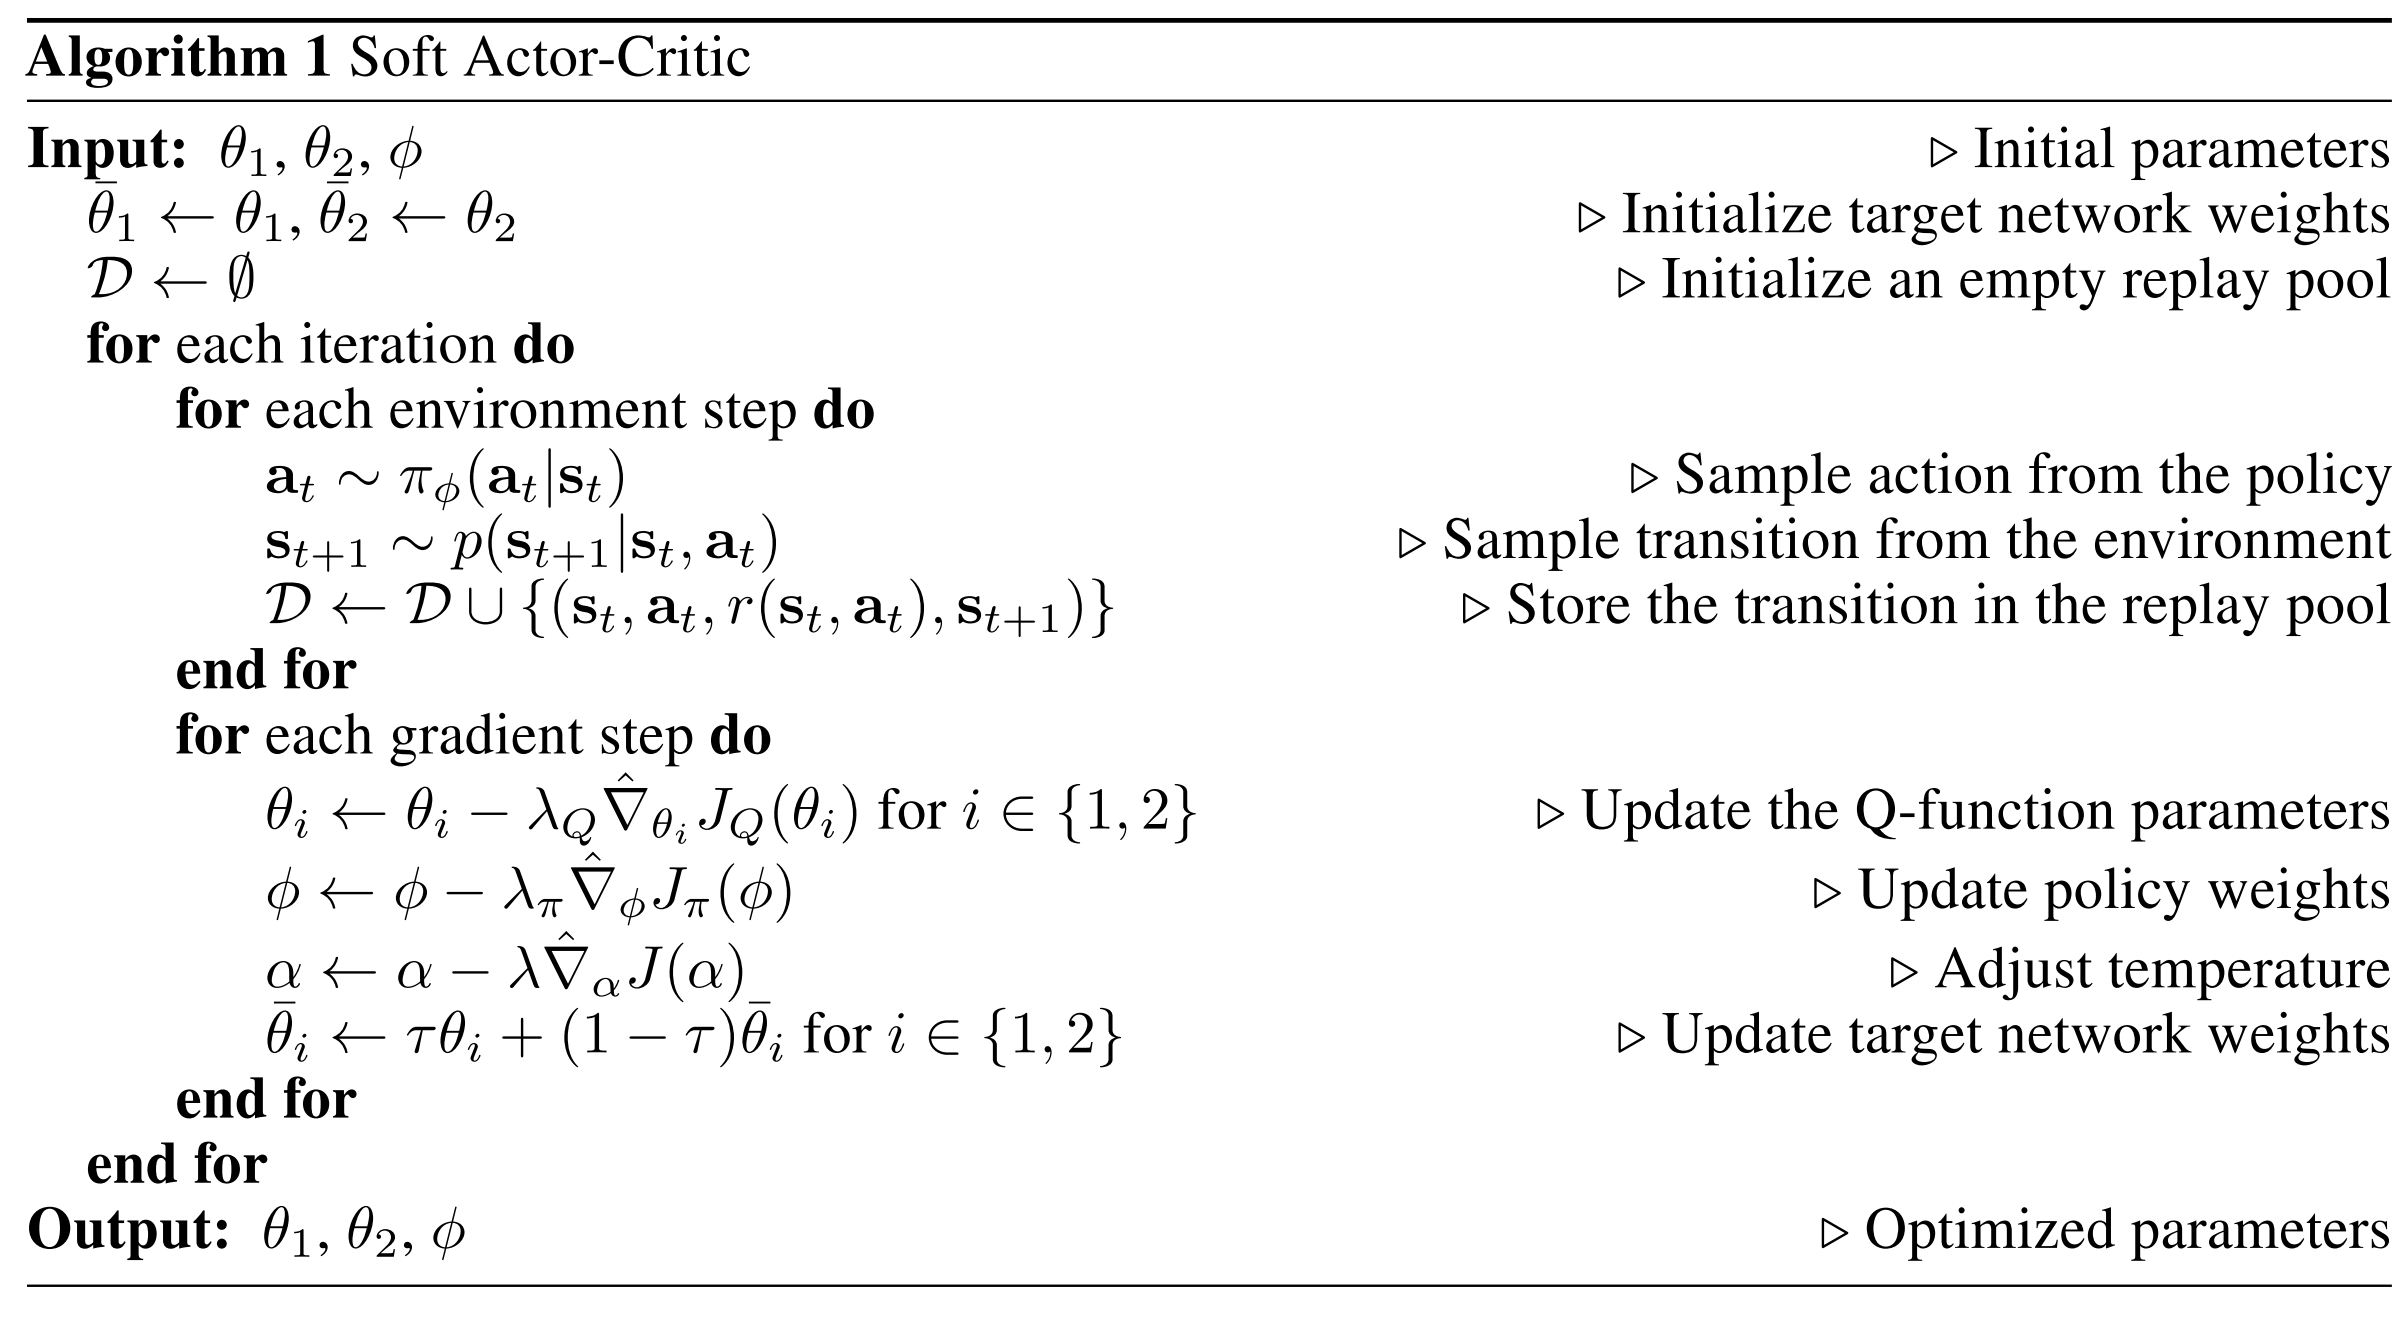
\includegraphics[width=1.0\textwidth]{figures/SACalgo}
    \caption{SAC pseudocode \cite{Haarnoja2018}}
    \label{fig:sacalgo}
\end{figure}

\section{Branching Dueling Q-Network (BDQ)}

\begin{figure}[htbp] 
    \begin{subfigure}{0.31\textwidth}
      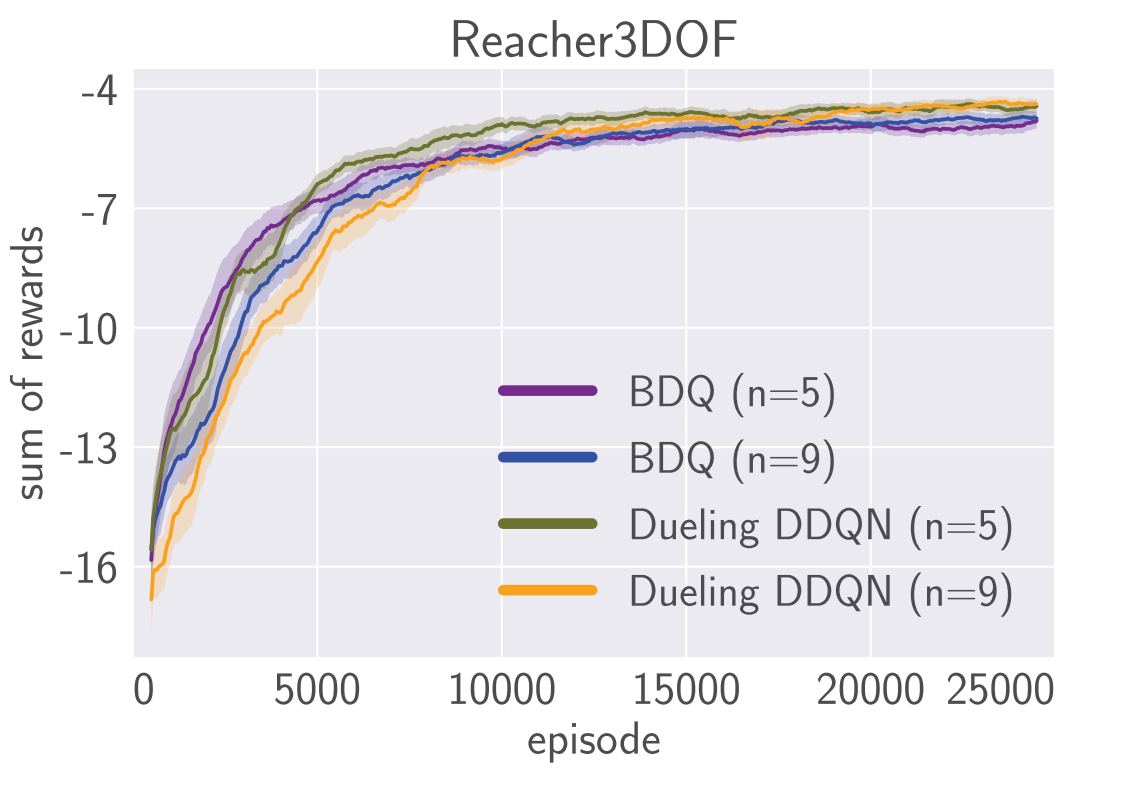
\includegraphics[width=\linewidth]{figures/BDQ1.png}
      \caption{} \label{fig:1a}
    \end{subfigure}%
    \hspace*{\fill}   % maximize separation between the subfigures
    \begin{subfigure}{0.31\textwidth}
      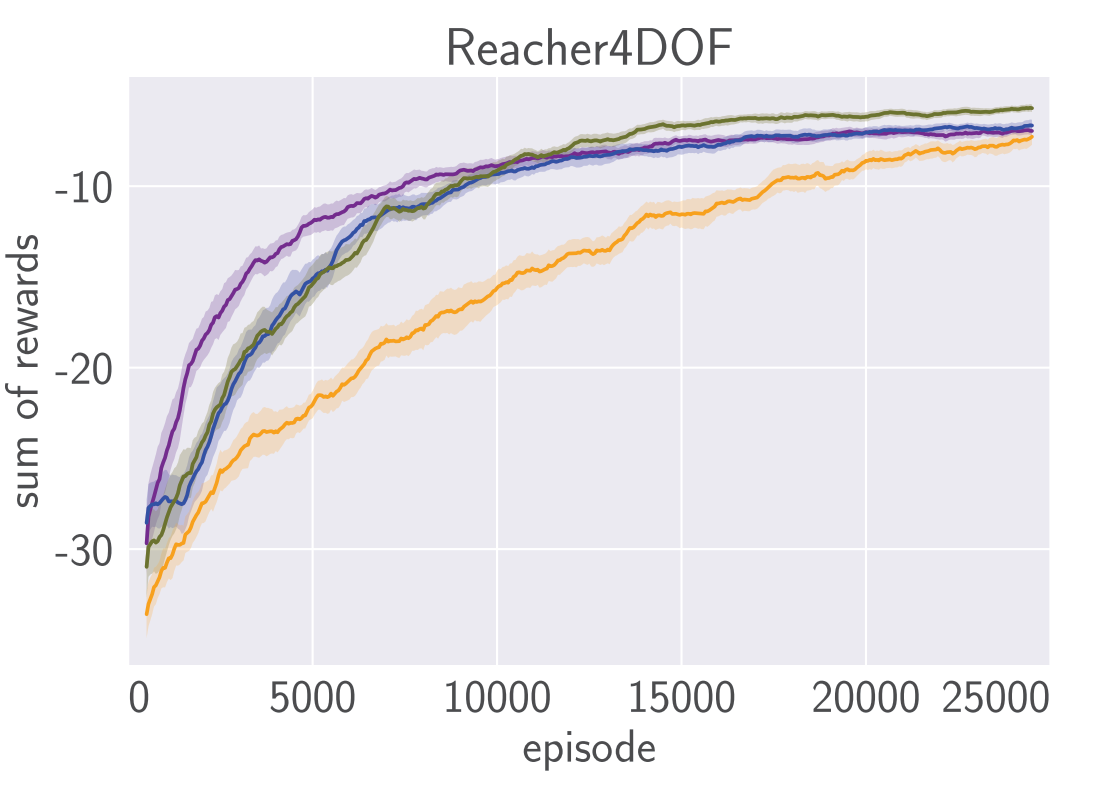
\includegraphics[width=\linewidth]{figures/BDQ2.png}
      \caption{} \label{fig:1b}
    \end{subfigure}%
    \hspace*{\fill}   % maximize separation between the subfigures
    \begin{subfigure}{0.31\textwidth}
      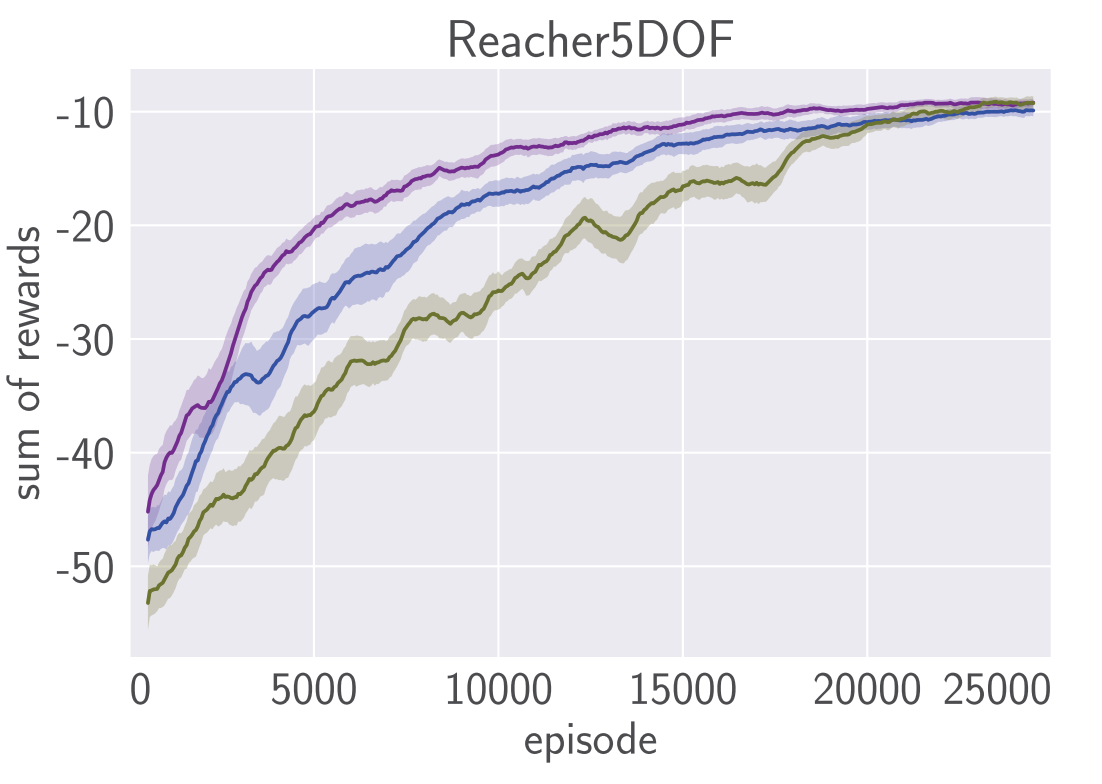
\includegraphics[width=\linewidth]{figures/BDQ3.png}
      \caption{} \label{fig:1b}
    \end{subfigure}%

\caption{BDQ performances compared to Dueling-Double-DQN with increasing action spaces \label{fig:BDQvsDDQN}}
\end{figure}

BDQ is our test algorithm. Tavakoli et al. developed BDQ as a variant of Dueling Double DQN \cite{Tavakoli2018}. They aimed to solve the intractability of the DQN algorithm on high dimensional continuous tasks. The key feature of their algorithm is the shared module. The shared module representation allowed the DQN algorithm to cope with the intractability problem. Tavakoli et al. showed that their network could output multi-dimensional actions without convergence issues. They believe the structure's stability is due to the encoded latent representation of the input in the shared module.

Their results stress that, especially in higher dimensional action spaces, BDQ performs better than Double-dueling DQN implementation \ref{fig:BDQvsDDQN}. Even compared to proven algorithms, like DDPG, BDQ performs better. Although researchers at Google DeepMind presented in 2016 that the DDPG algorithm outperforms DQN variants at almost every task \cite{Lillicrap2016}, Tavakoli et al. proved the opposite that BDQ shows better performance than DDPG on the Humanoid walking benchmark task \ref{fig:bdqvsddpg}.

\begin{figure}[htbp] 
    \centering
    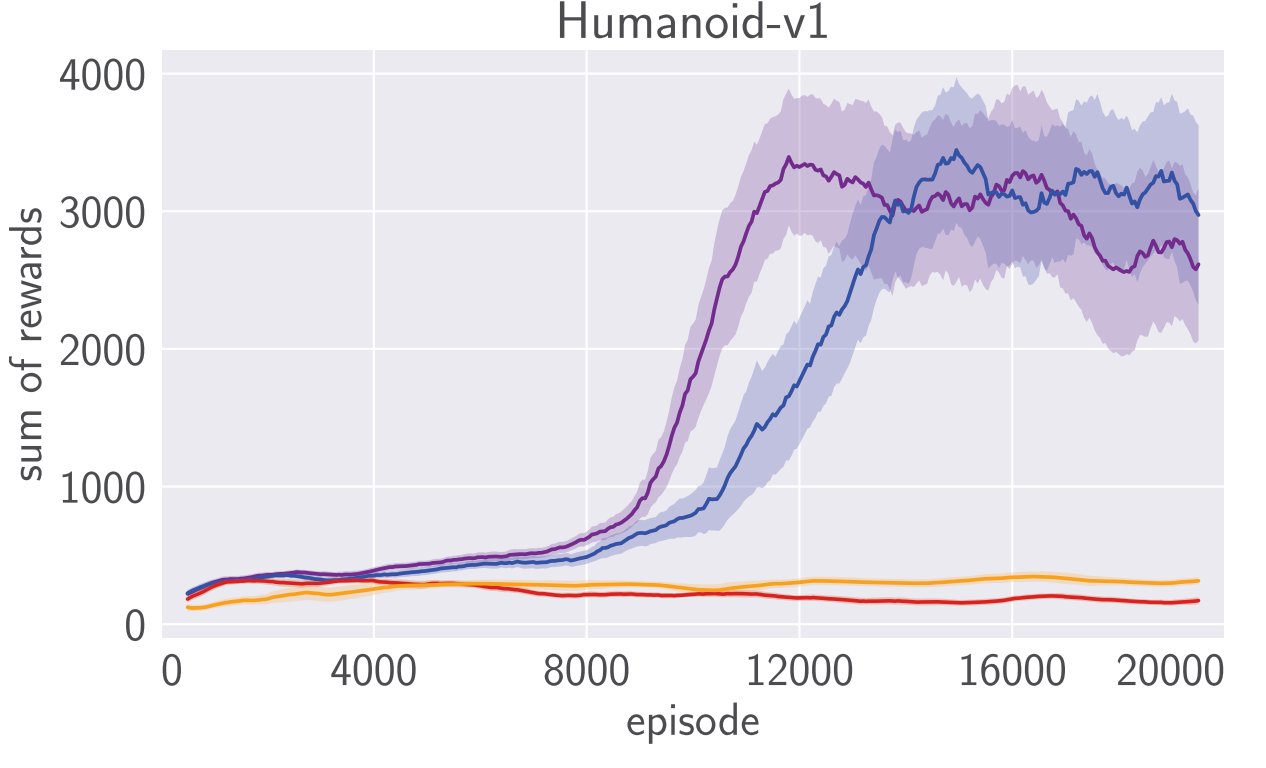
\includegraphics[width=0.7\textwidth]{figures/BDQvsDDPG}
    \caption{Blue and purple lines represent BDQ algorithm with 33 and 17 action padding. Orange line shows DDPG's performance}
    \label{fig:bdqvsddpg}
\end{figure}

In this section, we will go through the implementation details of BDQ. The authors of the BDQ article provided their implementation of BDQ on Github. Based on the original code and the insights from the article, we implemented our version of BDQ on stable-baselines codebase. As a result, we avoided the save, load model issues from BDQ original code, and welcomed new features such as callback structure, parameter manipulation, and warm starting. 


\subsection{BDQ Implementation}


\begin{figure}[htbp] 
    \centering
    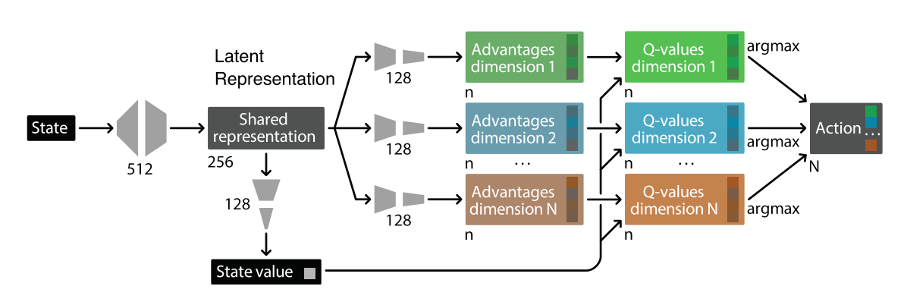
\includegraphics[width=1.0\textwidth]{figures/bdq_network.png}
    \caption{BDQ network representation}
    \label{fig:bdq_net}
\end{figure}

BDQ adopts new improvements from the DQN algorithm, such as double-q function, dueling architecture, prioritized replay. One crucial design decision is that while advantage functions are unique to every stream of actions, they kept the same state-value estimation for each action branch in  \ref{fig:bdq_net}. Later they combined the common state-value estimate and the advantage function in the aggregation layer. This approach helps with the generalization of similar states' actions by reducing the overfitting of action branches. Therefore, they can scale up to more complex and higher dimensional tasks, where Dueling-Double DQN becomes intractable.

Another key difference of BDQ is the aggregation layer; they subtract the mean advantage value from the individual branch's advantage value. Then, sum up the result to calculate the Q-function value of each branch, shown in \ref{eq:bdq_better}. Although the lack of identifiability problem exists, they achieve better results than the theoretically proven max reduction method(\ref{eq:bdq_proven}).

\begin{equation}
    Q_d(s, a_d) = V(s) + \Big(A_d(s, a_d) - \frac{1}{n} \sum\limits_{a_d'\in A_d}A_d(s, a_d')\Big)
    \label{eq:bdq_better}
\end{equation}


\begin{equation}
    Q_d(s, a_d) = V(s) + \Big(A_d(s, a_d) - \max\limits_{a_d'\in A_d}A_d(s, a_d')\Big)
    \label{eq:bdq_proven}
\end{equation}


TD-target definition of BDQ also differs from DDQN. Where DDQN based approach calculates the individual TD-target for every branch in \ref{eq:ddqn_tdtarget}, BDQ sets one global target for all actions by taking the mean of the max Q-function variable in the TD-target equation \ref{eq:bdq_tdtarget}. In our opinion, a common TD-target for all branches of BDQ underlines the dependency between action branches and forces them to act in collaboration.

\begin{equation}
    y_d = r + \gamma Q{_d^-}\Big(s', \arg\max\limits_{a_d'\in A_d}Q_d(s', a'_d)\Big)
    \label{eq:ddqn_tdtarget}
\end{equation}

\begin{equation}
    y = r + \gamma \frac{1}{N} \sum\limits_d Q{_d^-}\Big(s', \arg\max\limits_{a_d'\in A_d}Q_d(s', a'_d)\Big)
    \label{eq:bdq_tdtarget}
\end{equation}


Analogous to the TD-target definition, they express loss differently than the DDQN counterpart. BDQ authors calculate the loss first by taking the mean of the squared TD-error over the branches and then taking the expectation of this score in \ref{eq:bdq_loss}. Identical to the TD-target calculation, loss definition also helps the action branches to act dependent on each other.

\begin{equation}
    L = \mathop{\mathbb{E}}_{(s,a,r,s')\sim D} \Big[\frac{1}{N}\sum\limits_d(y_d-Q_d(s,a_d))^2]
    \label{eq:bdq_loss}
\end{equation}

The exploration-exploitation trade-off is still an on-going research in RL. Nevertheless, researchers assume that better-exploring algorithms have an edge over weakly exploring algorithms. SAC with a robust entropy-based exploration approach, considered to be the best exploring algorithm and the state-of-art RL algorithm \cite{Haarnoja2018}. BDQ original code offers two different exploration approach, epsilon greedy and Gaussian noise. Since epsilon-greedy usually used with discrete DQN based algorithms, the authors found it inadequate to explore continuous spaces. Instead of epsilon-greedy, they recommended the use of Gaussian noise for better performance.

BDQ follows the same pseudocode of double-DQN(\ref{fig:bdqalgo}) with dueling and branching network extensions.

\begin{figure}[htbp] 
    \centering
    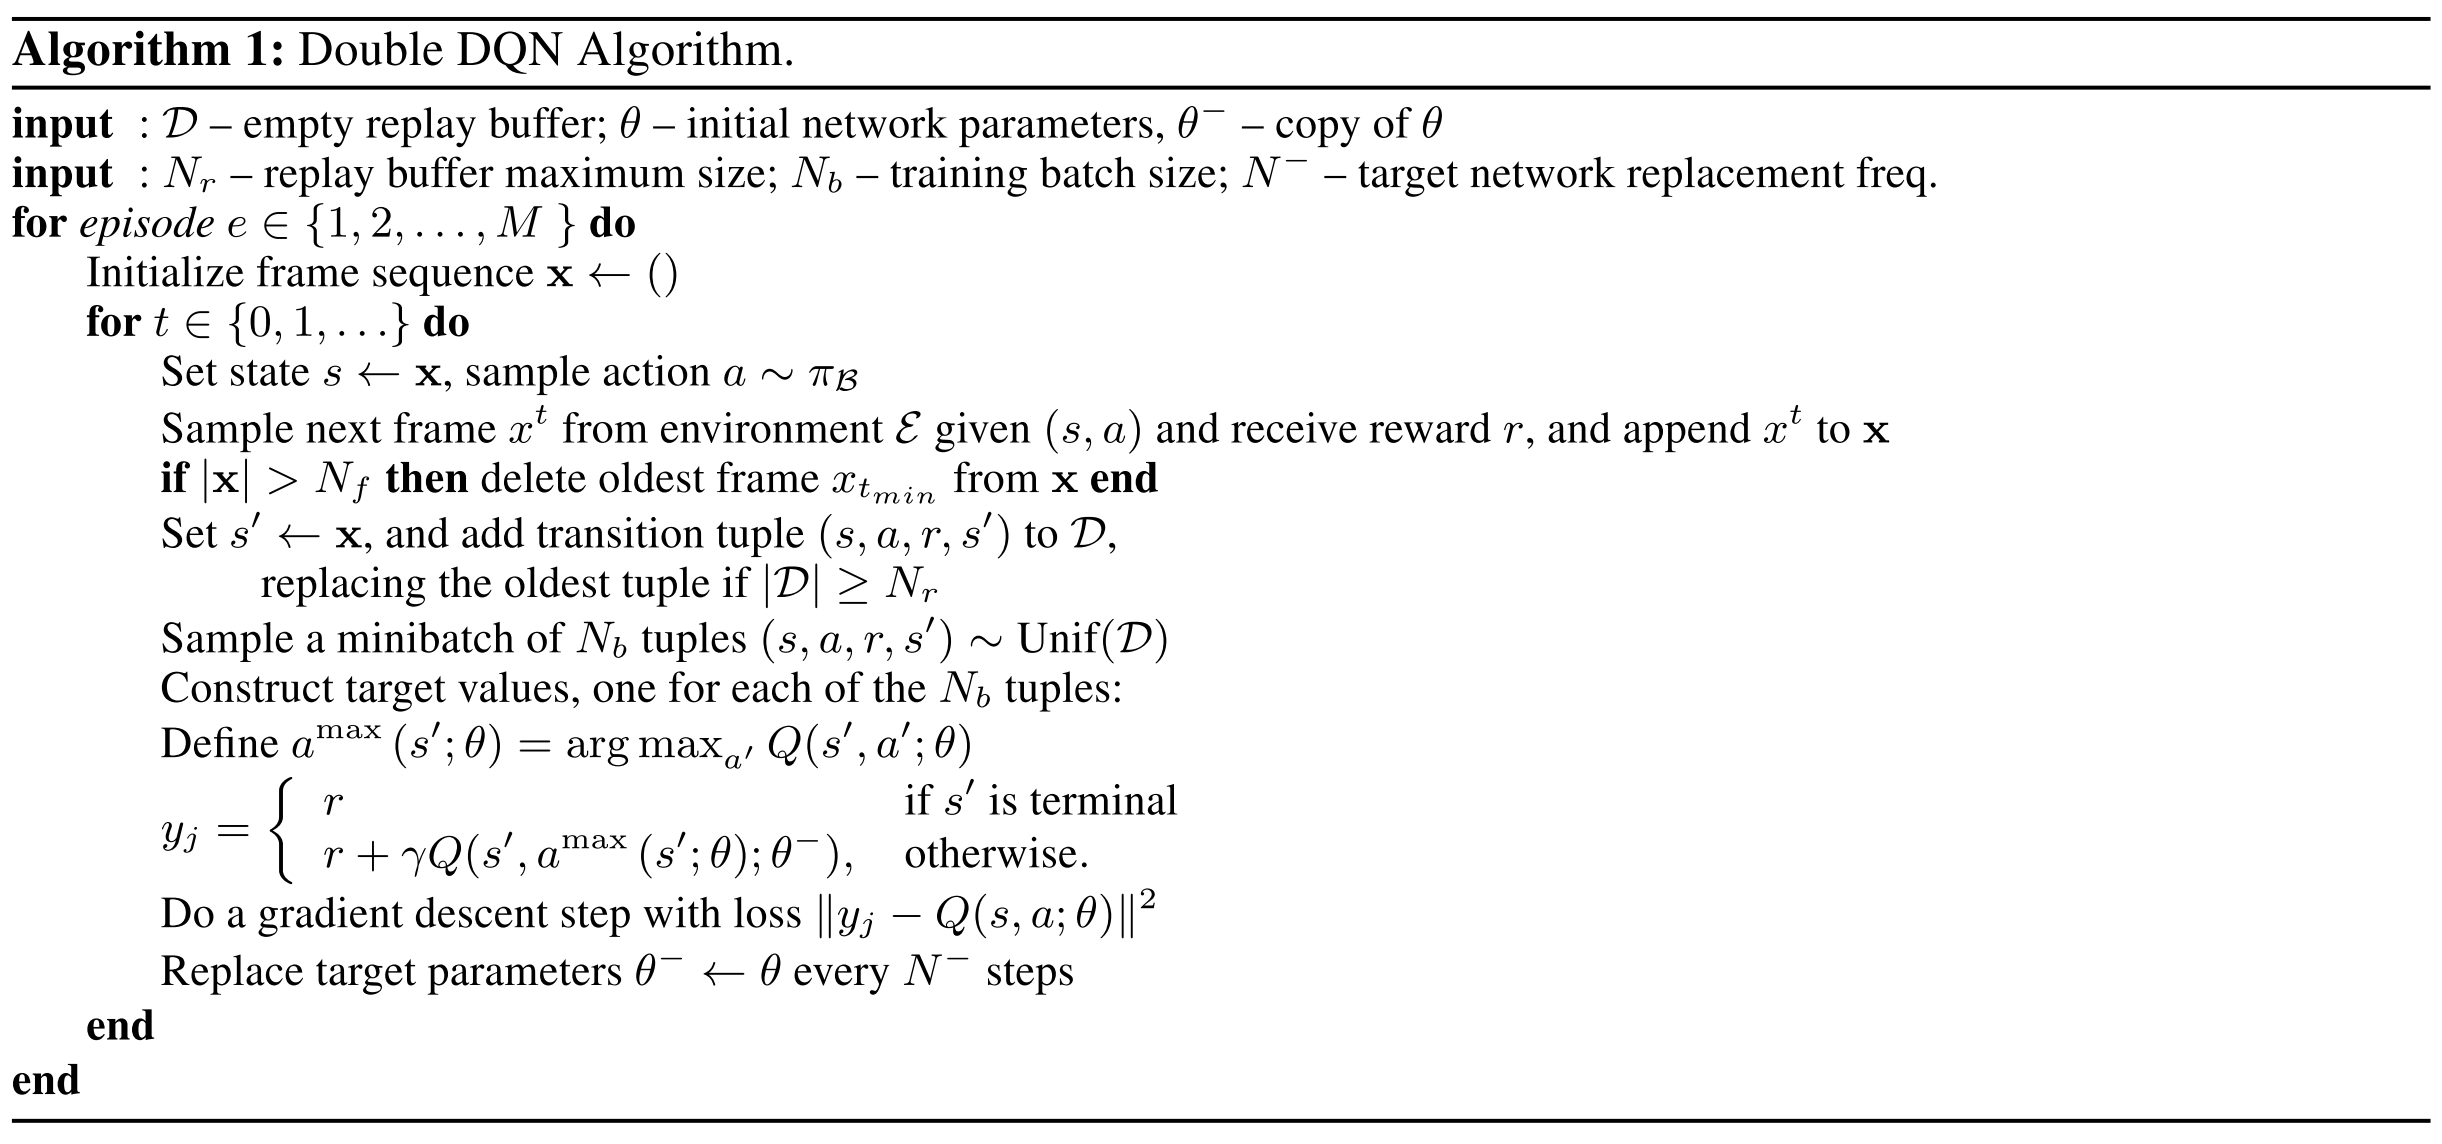
\includegraphics[width=1.0\textwidth]{figures/BDQalgo}
    \caption{Double-DQN pseudocode \cite{Wang2016}}
    \label{fig:bdqalgo}
\end{figure}
\section{OpenAI Gym}

The gym framework provides a standard definition of a reinforcement learning environment. It assumes that every environment is formalized with the Markov Decision Process (defined in section-\ref{section:markov}) \cite{OpenAIgym}. Hence, it follows the structure of the agent taking action and receiving observation and reward as a result of it.

\begin{figure}[htbp] 
    \centering
    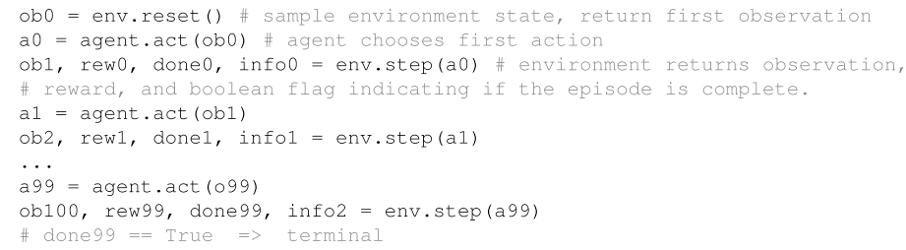
\includegraphics[width=1.0\textwidth]{figures/gyminterface}
    \caption{Gym interface to interact with an environment}
    \label{fig:gyminterface}
\end{figure}


The code example \ref{fig:gyminterface} demonstrates, the interaction between an agent and the environment. OpenAI designed the Gym framework in a way it is agent diagnostic. Therefore, it allows the user to try different algorithms on the agent side freely. The environment, on the other hand, should follow the Gym guidelines. A custom gym environment has to override the step, reset, seed, render, and close. Step function runs one timestep of the environment and returns a tuple of reward, observation, done, and info. Reset function resets the domain setting to a random or predefined initial state and returns the observation of that state. Seed function starts the seeding of the random number generator. Close function is called at the end when the user wishes to quit the environment. Thus, it performs the necessary memory clean-up or resource deallocation.

\begin{lstlisting}[language=Python, caption=Gym environment example instantiation, label=gymexample]
    from gym.envs.registration import register

    register(
        id='gripper-env-v0',
        entry_point='manipulation_main.gripperEnv.robot:RobotEnv',
    )

    env = gym.make('gripper-env-v0', config='config/gripper_grasp.yaml')
\end{lstlisting}

Gym environment definition also provides a useful helper gym.make function. After the registration of the custom environment, one can instantiate the environment with a simple one-liner represented in the code \ref{gymexample}. It also allows the user to pass an argument to the constructor of the custom environment. In our case, we provide the configuration file as an argument.
\section{Stable Baselines}


While the OpenAI gym framework identifies the environment, Stable Baselines provides the agent part of the RL framework. Stable Baselines is a robust open-source fork of OpenAI baselines. Yet it is based on OpenAI Baselines; it has surpassed the performance of OpenAI Baselines in many ways. 
The authors of Stable Baselines have composed a Medium article\footnote{\url{https://bit.ly/3ia3GvM}} that describes every additional feature and bug fix over OpenAI baselines. In this section, we will only mention the critical components that are needed for our project.

First and foremost, Stable Baselines has strong support for the state-of-art algorithm SAC. SAC proved to be the best algorithm we tested in our environment. Apart from SAC, it supports ten more algorithms\footnote{a2c, 
acer, acktr, ddpg, dqn, gail, her, ppo, trpo, td3}. Stable Baselines maintains a sophisticated save/load structure. Since we aim to warm-start and fine-tune the neural network variables, we should save and load the network variables individually. A use-case in our application is truncating the last soft-max layer of a saved model to change the action-space size. We often encountered problems with OpenAI Baselines save/load structure.

Moreover, Stable Baselines supports input and reward normalization. Later in the results section, we will show that our best performing model is equipped with both input and reward normalization.

Lastly, because of the extra features, fully documented, and tested code-base, we decided to reimplement the BDQ algorithm on Stable Baselines. Example of how to run a simple training and saving can be seen below in \ref{list:sb_bdq}


\begin{lstlisting}[language=Python, caption=Example of training and saving BDQ algorithm on gripper-env, label=list:sb_bdq]
    import gym

    from stable_baselines.bdq.policies import MlpActPolicy
    from stable_baselines import BDQ

    env = gym.make('gripper-env-v0', config='config/gripper_grasp.yaml')

    model = BDQ(MlpActPolicy, env, verbose=1)
    model.learn(total_timesteps=10000)

    obs = env.reset()
    for i in range(1000):
        action = model.predict(obs)
        obs, rewards, dones, info = env.step(action)
    
    env.close()
\end{lstlisting}
\section{Machine Learning Framework}


RL owes its success partly to a strong function approximator, deep neural networks. Where tabular Q-function only solved games like tic-tac-toe, neural networks integration to Q-function scales to high dimensional complex tasks like Atari games \cite{Mnih}. The growing success of neural networks inspired large companies like Google and Facebook to start their own open-source machine learning frameworks. Among those projects, Tensorflow, Keras, and PyTorch are the most popular ones \cite{Tensoflow} \cite{Keras} \cite{PyTorch}. 

Granted that we decided to work with Tensorflow and Keras on different parts of the project, it is worth mentioning that PyTorch is becoming dominant in research \cite{Horace}. In figure \ref{fig:ptvstf} demonstrates how Pytorch has risen steeply in terms of mentions in the major conferences. It achieved a staggering comeback from a maximum of \(6\%\) mentions to \(78.72\%\) mentions in three years.  

\begin{figure}[htbp] 
    \centering
    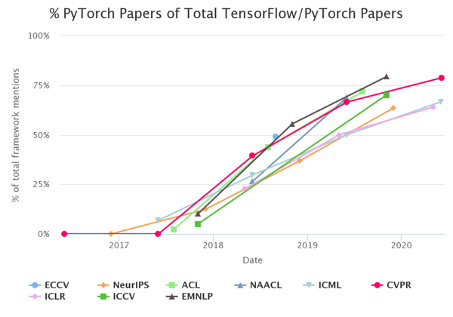
\includegraphics[width=0.7\textwidth]{figures/tfvspytorch}
    \caption{PyTorch and Tensorflow comparison based on the mentions in major machine learning conferences \cite{Horace}}
    \label{fig:ptvstf}
\end{figure}


According to the researchers, PyTorch's success is due to simplicity, great API, and performance. Even Tensorflow, in its last edition Eager, delivered a similar API to PyTorch. Though, there have been reports about the weaknesses of Eager in performance and memory. In short, it is unlikely that Tensorflow recovers and catches PyTorch anytime soon.

In conclusion, it is also possible to see the transition from Tensorflow to Pytorch in the RL community. Stable Baselines released the PyTorch version of Baselines algorithms in May 2020 \cite{stable-baselines3}. OpenAI Spinningup, an educational incentive for RL teaching from OpenAI, has moved to PyTorch in February 2020. Furthermore, they now host the master branch with PyTorch implementation \cite{SpinningUp2018}.

 
% \input{chapters/reinforcement_learn/libraries.tex}